\subsection{The process of formulating Phase 2 recommendations}\label{ssec:process}

%The current recommendations presented here constitute ``Phase 2'' of the LSST strategy optimization process and substantially narrow the parameter space of the possible LSST strategy options. 

To converge to the recommendations presented herein, the SCOC has reviewed close to 500 simulations (v2.X) and hundreds of metrics, including metrics evaluating the impact of the cadence choices on the system, compliance with the \citepalias{LPM-17}, and performance on community-contributed science goals. The simulations were released in batches starting in November 2021, and they are described in detail in a  community.lsst.org post\footnote{\url{https://community.lsst.org/} is an online form used by Project for discussions and announcements. The specific post describing the v2.X simulations is \url{https://community.lsst.org/t/survey-simulations-v2-1-april-2022/6538}} and on GitHub.\footnote{\url{https://github.com/lsst-pst/survey_strategy/blob/main/fbs_2.0/SummaryInfo_v2.1.ipynb}}

After reviewing \opsim\ v2.X, the SCOC commissioned the production of and reviewed $\sim 10$ simulations (\opsim\ version v2.99) that largely straddled the remaining survey strategy options. An initial set of four simulations were released on October 24, 2022\footnote{\url{ https://community.lsst.org/t/draft-of-v3-0-survey-strategies-v2-99/7159}} and were presented at the Third SCOC-Science Collaborations Workshop on November 2-3, 2022.\footnote{\url{https://project.lsst.org/meetings/scoc-sc-workshop3/home}.}  Additional simulations refined the v2.99 initial set of four and implemented suggestions collected during and after the November 2022 workshop. Among those simulations, we selected the one that best represents our current recommendation as \texttt{baseline\_v3.0} (described in \autoref{sec:v3})

The detailed process of reviewing input and converging to an optimal recommendation is complex, because, in this context, ``optimal'' is difficult to define. While this process of generating survey simulations and associated metrics does provide quantitative measures of enhancement of the survey, it should be noted that the metrics are not always directly comparable, nor is the overall importance of the science they reflect an objectively measurable quantity, such that a purely numerical optimization process is not possible. The performance of the strategy on different science drivers has to be balanced in the light of (1) the output of available metrics, but also (2) expert considerations about the relative importance of the performance gain/loss for different science drivers, (3) the significance of the performance change (\emph{i.e.} the metrics are not ``standardized'' in a collective sense as they measure quantities with different units and that may not be directly comparable), and (4) how core a science goal is to the overall Rubin LSST science endeavor. At a high level, the SCOC reviews the increase/decrease in performance for a science case as compared to the earlier LSST plans, known as the ``baseline'' (in the case of the Phase 2 recommendations, comparing the \texttt{v2.0} and \texttt{v2.1} simulations with the \texttt{baseline\_v1.7}, and  the simulations that implement the current recommendations ---\texttt{v2.99} and \texttt{v3.0}--- with \texttt{baseline\_v2.X}). Generally, performance changes on metrics greater than a few percent are regarded as significant. Further refinement is beyond the current scope of the SCOC work, particularly considering the as-of-yet unknown performance of the system as built. Finally, the process of optimizing the survey is further complicated by the fact that the SCOC is provided with LSST families of simulations that aim to stretch the survey in one or another direction (\emph{e.g.}, modifying the footprint or the rolling scheme). This is typically done in isolation, but the SCOC needs to keep track of and balance the compound effects of survey changes across multiple parameters, which might significantly impact a science case even when individually they had a small effect. 

The SCOC does not only review the MAF metrics performance but also provides \emph{key interpretability} to the metrics and their performance. For this the SCOC is composed of experts in different domains, attempting to cover all science areas relevant to Rubin. It should be noted, however, that SCOC members are explicitly instructed not to view themselves as advocates of specific science areas, but rather as members exercising their best judgment on the LSST observing strategy with the goal of maximizing the \emph{overall} scientific throughput of the survey.

The SCOC has also liaised with the eight Science Collaborations (SCs) of LSST, with 1--3 members of the SCOC assigned to each SC as liaisons.\footnote{See \url{https://www.lsst.org/content/charge-survey-cadence-optimization-committee-scoc} for the full list of SCOC liaisons.} In this role, SCOC members are charged with enabling and ensuring a bidirectional communication flow between the SCOC and the SCs. 

The SCOC is committed to transparency. Communication between the SCOC and the community is made through a number of channels: via liaisons to the SCs; summaries of the SCOC goals and discussions on community.lsst.org;\footnote{See the dedicated ``Survey Strategy'' topic (\url{https://community.lsst.org/c/sci/survey-strategy/37}).} presentations of our current work and status of the recommendations at relevant meetings, including the annual Project Community Workshop (PCW); and by organizing dedicated workshops to come together with the community. Most recently the SCOC and community met in the Third SCOC Workshop on November 2-3, 2022.\footnote{\url{https://project.lsst.org/meetings/scoc-sc-workshop3/home}.} Phase 2 recommendation updates have been released in a post on community.lsst.org\footnote{\url{https://community.lsst.org/t/scoc-v2-0-and-2-1-simulations-review-timeline/6712}.} leading to the November workshop, including short summaries of the discussion as conducted in each full SCOC meeting.\footnote{Released in \url{https://community.lsst.org/t/scoc-v2-0-and-2-1-simulations-review-timeline/6712}.} Starting in November 2022, a dedicated community post is regularly updated with meeting summaries and future meetings' schedules,\footnote{\url{https://community.lsst.org/t/public-scoc-meeting-minutes/7185}.} and regular office hours have been established.\footnote{\url{https://community.lsst.org/t/scoc-office-hour/7221}.}

While we had solicited official reports in the SCOC Phase 1 deliberations (the 2019 Cadence notes,\footnote{See \autoref{fn:cnotes}.}
the SCOC decided shortly after the v2.0 simulations were made available {\it not} to solicit formal reports from the SCs and the community in the Phase 2 deliberations so as to avoid overburdening the community members. Yet several SCs shared their feedback in a number of written reports. Reports received by the SCOC in its Phase 2 deliberations include analyses of the \opsim\ via metrics relevant to a specific science-focused group, as well as  considerations not based on metrics but on expert opinions from domain scientists. All these reports are made available to the reader.\footnote{Listed in the order in which they were received, these include reports from the
SSSC (May 2022);
the TVS and SMWLV SCs (a report on Galactic science and a more specific report on microlensing), TVS SC (on exctra-galactic science), and TVS and AGN SCs (the latter four all first received in March 2022); three 
DESC reports (June 2022, October 2022, and November 2022); a report from the AGN SC (August 2022); all these reports are available on the SCOC website at \url{https://lsst.org/content/reports-scs-v2x-simulations}.} Feedback delivered to the SCOC in the form of written reports, through interactions on community.lsst.org,\footnote{Including the thread \url{https://community.lsst.org/t/scoc-v2-0-and-2-1-simulations-review-timeline/6712}.} as well as reported by the SCOC liaisons was considered and incorporated in our decision-making process. 


As discussed above, the comparison of results of the metrics, hereafter referred to as metrics or MAFs, produced by the Survey Strategy team (primarily to assess compliance with the SRD and other system requirements) and by the community constitute a quantitative ---or at least quantifiable--- feedback on LSST simulations. Three kinds of plots are generally produced to compare the performance of simulations for sets of MAFs.

\begin{itemize}

\item {\bf Radar Plots:} helpful to review and compare small numbers of simulations and small numbers of metrics. In a radar plot such as \autoref{fig:radar} each vertex corresponds to a MAF, and each simulation is indicated in a different color. By design, the reference simulation forms a ``perfect'' circle, where the performance for each MAF is =1. For a given simulation, a MAF performance that extends outward (inward) of the reference circle indicates an improvement (decrease in) performance. 

\begin{figure}[h!]
\centering
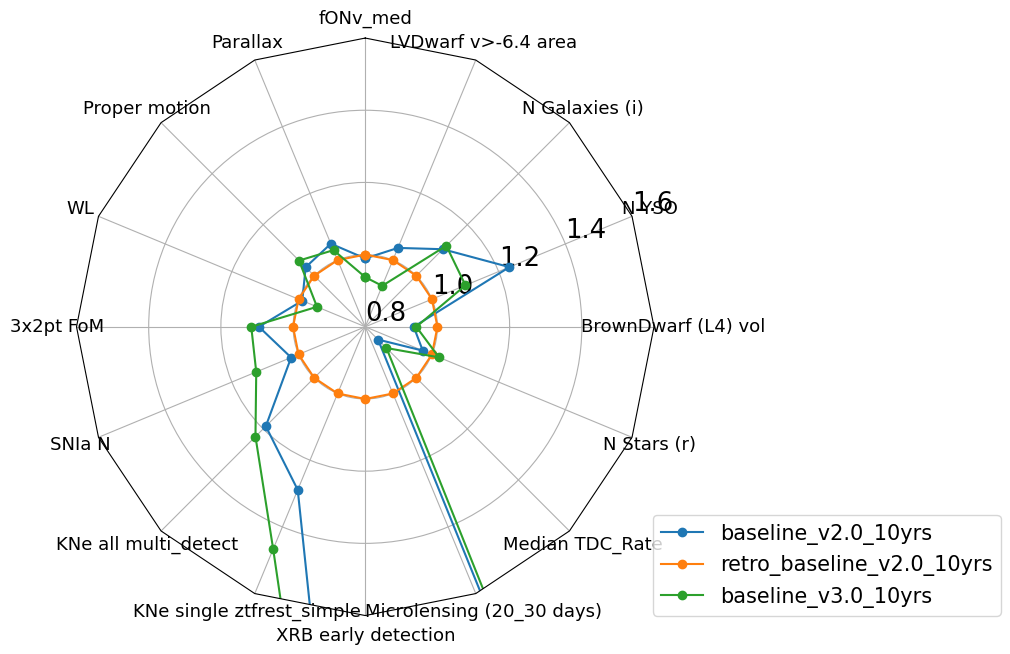
\includegraphics[height=0.4\textwidth]{figures/SCOC299radar1.png}
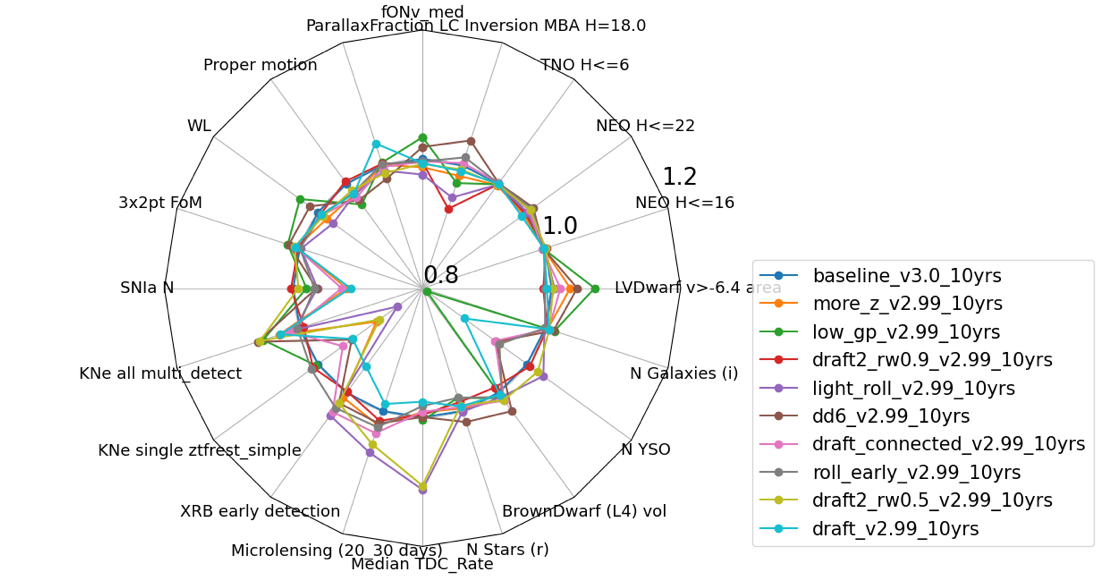
\includegraphics[height=0.4\textwidth]{figures/SCOC299radar2.png}
\caption{Radar plots comparing  \texttt{baseline\_v3.0} with earlier baseline simulations (\emph{top}) and the v2.99 simulations released starting on October 24th, 2022 with \texttt{baseline\_v3.0} (\emph{bottom}) . The majority of the metrics considered display improvements compared with earlier baseline simulations. The improvement on the ``XRB early detection'' and ``Microlensing (20\_30 days)'' metrics is $>300\%$ between \texttt{baseline\_v3.0\_10yrs} and \texttt{retro\_baseline\_v2.0\_10yrs} which reproduces baseline \texttt{baseline\_v1.7\_10yrs}, and extend outside of the range of the plot.}\label{fig:radar}
\end{figure}
\FloatBarrier

\item {\bf Heatmaps}: Larger collections of metrics and simulations are generally better visualized with heatmaps (see \autoref{fig:heatmap}), where families of simulations (as columns) and families of MAFs (as rows) can be grouped together by appropriate ordering. 


\begin{figure}[t!]
\centering
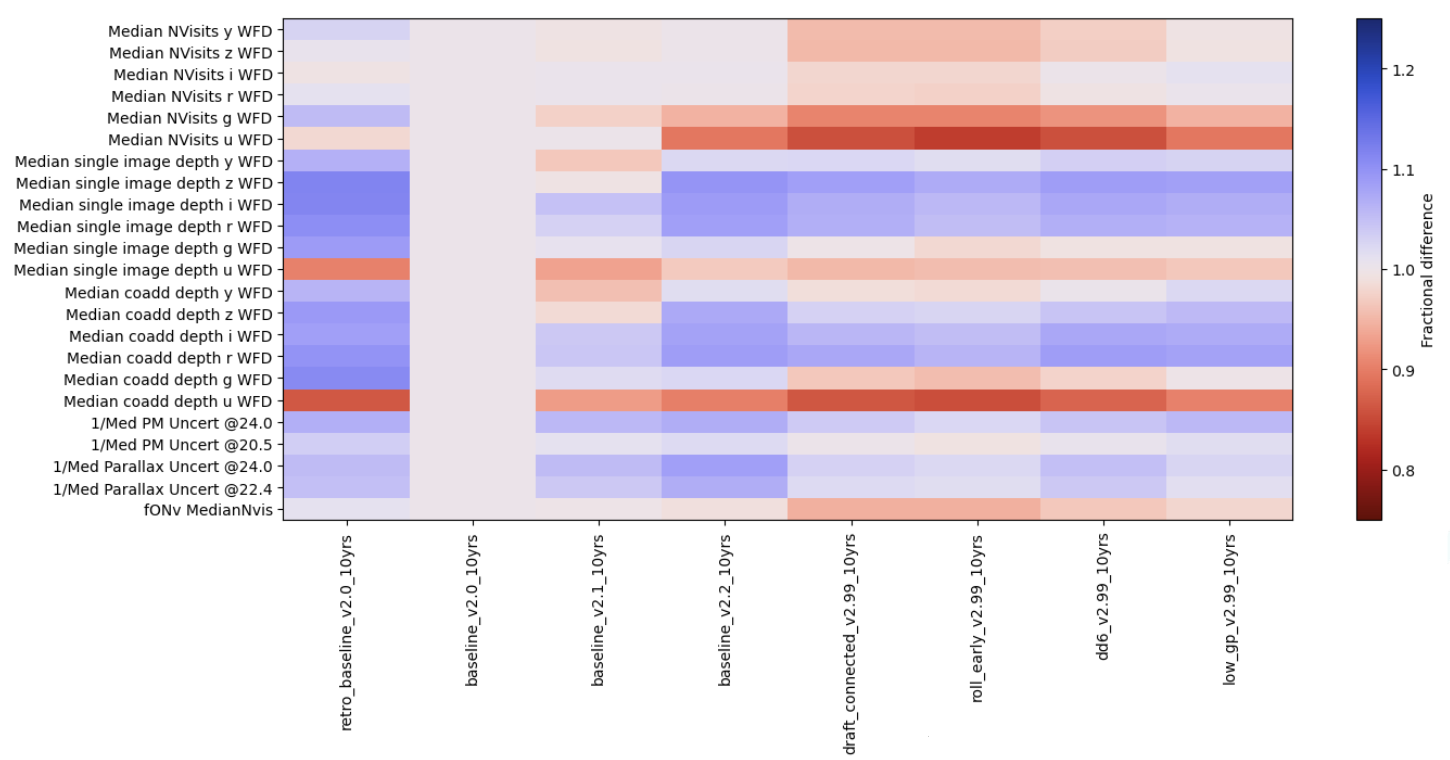
\includegraphics[width=0.8\textwidth]{figures/SCOC299heatmap1.png}
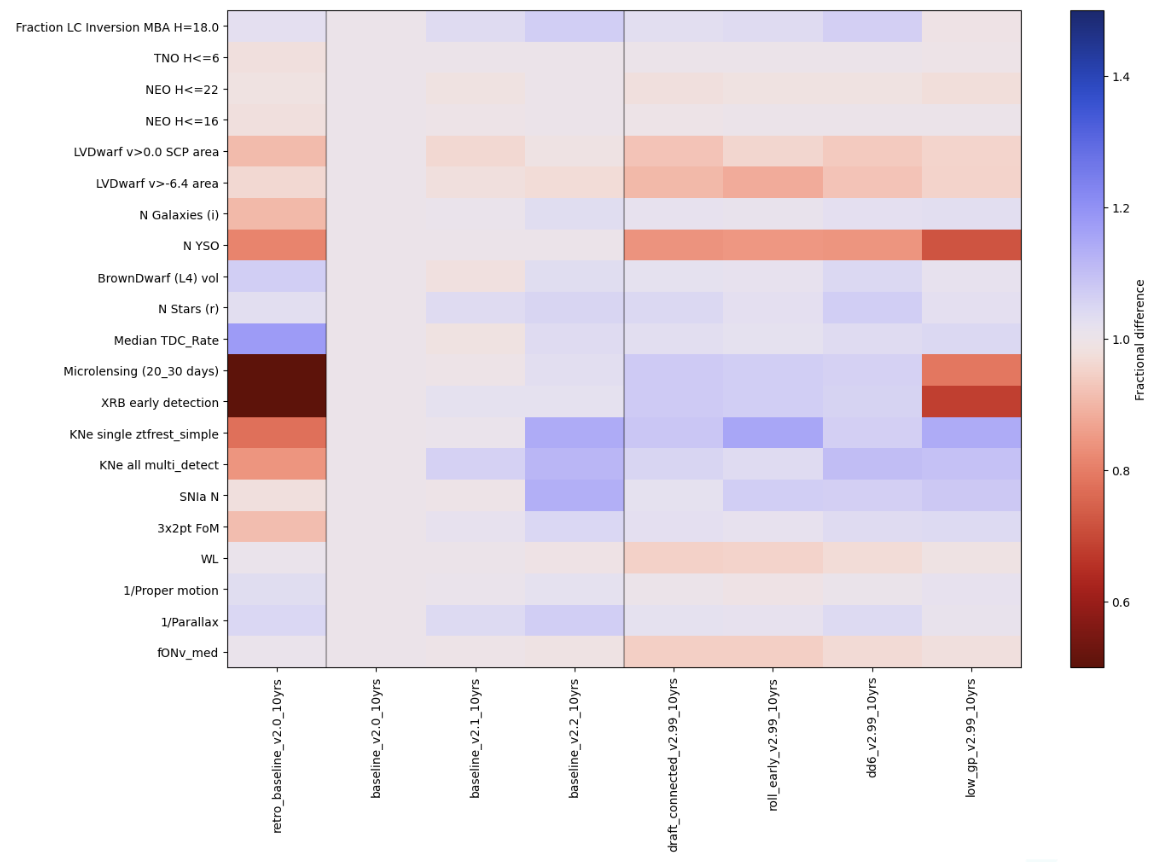
\includegraphics[width=0.8\textwidth]{figures/SCOC299heatmap2.png}
\caption{Heat maps comparing the first four v2.99 simulations (released on October 24th, 2022)  with earlier baselines for a selection of system metrics (\emph{top}) and science metrics contributed by the community (\emph{bottom}). Blue blocks indicate improvements compared to a reference simulation (here \texttt{baseline\_v2.0\_10yrs}), and red ones indicate performance loss. The increase or drop of a series of MAFs in adjacent rows may indicate a systemic problem. For example, the SCOC noticed and investigated the decrease in Galactic and Local Volume performance as measured by the number of dwarf galaxies and Young Stellar Objects (YSO) with the help of the SMWLV SC and TVS SC.}
\label{fig:heatmap}
\end{figure}
\FloatBarrier


\item {\bf Line plots}: 
While heatmaps provide a synoptic view, the amount of gain/loss is not obviously quantifiable via the color intensity. Line plots are useful to inspect small numbers of (typically related) MAFs and provide quantifiable significance of a gain/loss (see \autoref{fig:lineplot}). 


\end{itemize}
\begin{figure}[h!]
\centering
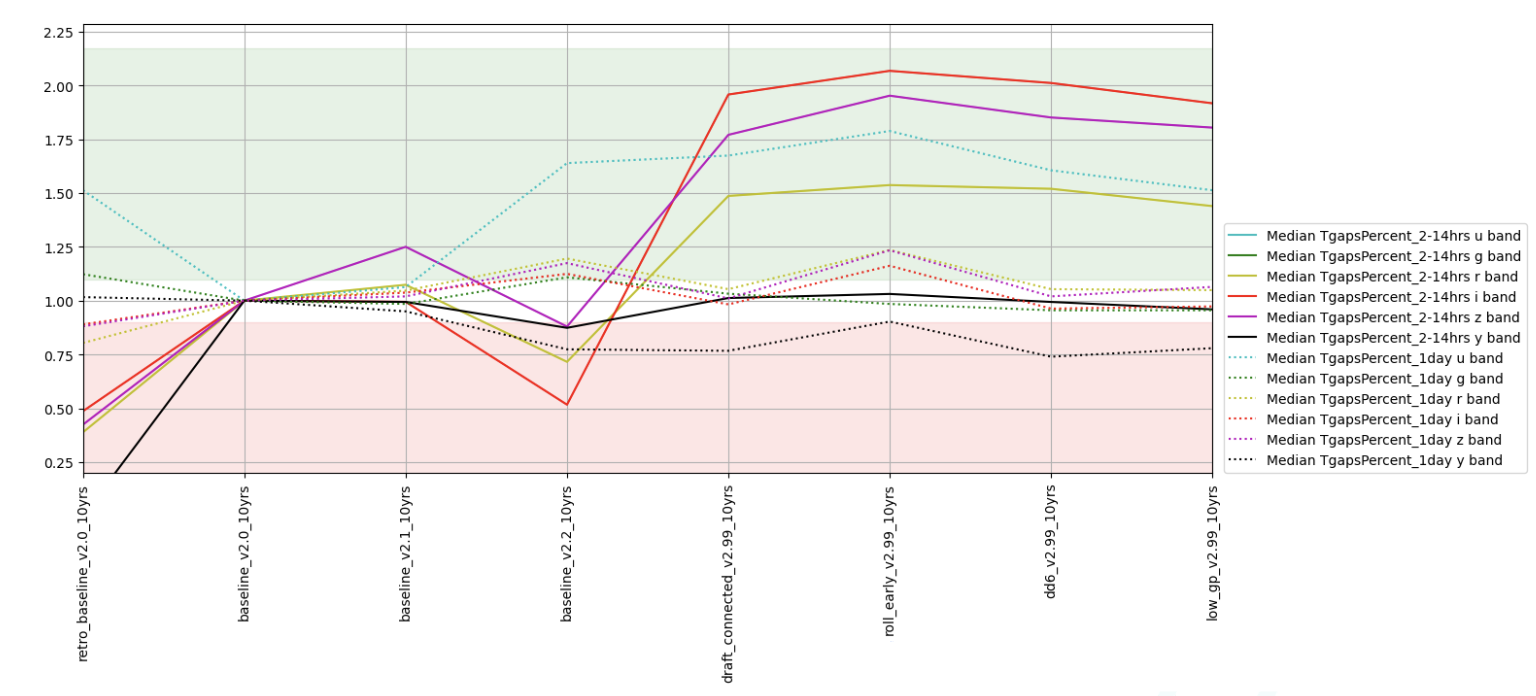
\includegraphics[width=0.99\textwidth]{figures/SCOC299lines.png}
\caption{A line plot showing the performance of metrics measuring intra-night cadence for the same simulations used in \autoref{fig:heatmap}: each MAF measures coverage on specific time scales. All values are to be compared with 1, the performance of a reference simulation (here \texttt{baseline\v2.0\_10yrs}). The shaded areas indicate potentially significant performance changes, generally set to a $>5\%$ performance difference. The SCOC notes a generally improved performance for nearly all the v2.99 Time Gap metrics, with performance gains as high as 100\% in some cases.}
\label{fig:lineplot}
\end{figure}

\FloatBarrier
The survey strategy team makes these visualizations available via jupyter notebooks organized by simulation family, MAF family (including notebooks specifically designed for an interest group or SC), and SCOC question (see below). All these notebooks are available on GitHub.\footnote{\url{https://github.com/lsst-pst/survey_strategy}.}



\subsection{Open questions addressed in Phase 2}\label{sec:synopsis}

The SCOC has organized its Phase 2 deliberation around eight topics (posted on community.lsst.org\footnote{\url{https://community.lsst.org/t/scoc-v2-0-and-2-1-simulations-review-timeline/6712} and listed at the end of this section.} in June 2021). Many of these topics came from questions that were addressed to some extent in Phase 1 but needed further study. The open questions and remaining SCOC tasks identified in earlier reports (\citeds{PSTN-051, PSTN-053}) were systematically explored in the \texttt{v2.0}, \texttt{v2.1}, and \texttt{v2.2} series of \opsim\ LSST simulations\footnote{The simulations were described in \url{https://github.com/lsst-pst/survey_strategy/blob/main/fbs_2.0/SummaryInfo_v2.1.ipynb} and on community.lsst.org \url{https://community.lsst.org/t/survey-simulations-v2-1-april-2022/6538}.} and include:

%Here we report the questions considered within each topic and the information and deliberations that led to the SCOC recommendations encapsulated in the \texttt{v2.99} and \texttt{baseline\_v3.0} simulations are described in detail in the next section.

\begin{itemize}
\item Establish final survey footprint definitions (\emph{e.g.}, the exact Declination and dust extinction limits for the WFD region, the exact definition of the Galactic bulge region),
\item Decide which sets of filters should be used in sets of visits,
\item Decide the exposure duration and the number of visits in the $u$ band,
\item Optimize further the rolling cadence implementation,
\item Optimize further the DDF cadences.

\end{itemize}

The members of the SCOC further refined the scope of each question and split into eight overlapping subgroups to review the Rubin- and community-contributed metrics relevant to each topic, jointly with community feedback on the simulations. 
The goal of these subgroups was to formulate an initial recommendation to be presented to, reviewed by, and agreed upon by the whole SCOC. Subgroup presentations were distributed over the months of June through August 2022, with the majority of the subcommittee presenting and leading discussions on their recommendations ahead of the August 2022 PCW, where these preliminary recommendations were presented.\footnote{\url{https://project.lsst.org/meetings/rubin2022/agenda/survey-strategy-i}.} Further refinement of the full SCOC deliberations and further review of the recommendations resumed in mid-September 2022.

The eight subcommittees of the SCOC  and the topics they were tasked to address are:
\begin{enumerate}
\item{Early Science} (\autoref{q:Early})

\item{Footprint} (\autoref{q:Footprint})

\item{Filter Distribution} (\autoref{q:Filters})

\item{Nightly Visits pairs and triplets} (\autoref{q:Visits})

\item{Rolling Cadence} (\autoref{q:Rolling})

\item{DDF Strategy} (\autoref{q:DDF})


\item{Microsurveys} (\autoref{q:Micro})

\item{Time allocation for ToO} (\autoref{q:ToO})

\end{enumerate}

In the following section (\autoref{sec:rec}) we describe in detail the deliberation process for each of these eight topics and the associated SCOC Phase 2 recommendation. In \autoref{sec:v3} we describe the \texttt{baseline\_v3.0} simulation that implements our current recommendations. In \autoref{sec:refinements} we highlight the elements of the current recommendation that need further refinement.
